\documentclass[a4paper,12pt]{article}

\usepackage[T2A]{fontenc}
\usepackage[utf8]{inputenc}
\usepackage[english,russian]{babel}
\usepackage{amsmath}
\usepackage{geometry}
\usepackage{graphicx}
\usepackage[section,above,below]{placeins}
\usepackage{afterpage,placeins}
\usepackage{booktabs}
\usepackage{listings}
\usepackage{color}

\usepackage{algorithm}
\usepackage[noend]{algpseudocode}

\DeclareGraphicsExtensions{.png,.jpg}

\geometry{left=2cm}
\geometry{right=1.5cm}
\geometry{top=1cm}
\geometry{bottom=1.5cm}

\headheight = 1cm
\footskip = 0pt
%\usepackage[left=20mm, top=10mm, right=10mm, bottom=5mm, nohead, nofoot]{geometry}

\parskip = 4.25mm % расстояние между строками
\parindent=6.375mm % расстояние между абзацами
\floatname{algorithm}{Алгоритм} % переопределение имени в псевдокоде

%\renewcommand\[{\begin{equation}}
%\renewcommand\]{\end{equation}}

\begin{document}

    \begin{titlepage}

        \begin{center}
            \large
            Государственное образовательное учреждение высшего профессионального образования\\
            “Московский государственный технический университет имени Н.Э.Баумана”
            \vspace{3cm}
            
            \textsc{Дисциплина: Анализ алгоритмов}
            \vspace{0.5cm}
                
            \textsc{Лабораторная работа №1}
            \vspace{3cm}
            
            {\LARGE Расстояние Левенштейна}
            \vspace{3cm}
            
            Студент группы ИУ7-54Б,\\   
            Котов Никита
            \vfill
            
            2019 г.
            
            \end{center}
    \end{titlepage}
    
    \begin{center}
    	\tableofcontents
    \end{center}
	
	\setcounter{page}{2}
	\newpage
    \begin{center}
        \section*{Введение}
        \addcontentsline{toc}{section}{Введение}
    \end{center}
        \label{sec:intro}
\qquad Расстояние Левенштейна определяет, сколько раз необходимо добавить/удалить/заменить символ, чтобы одну строку превратить в другую.
        
Впервые задачу упомянул в 1965 году советский математик Владимир Иосифович Левенштейн при изучении последовательностей\cite{litlink5}. Впоследствии более общую задачу для произвольного алфавита связали с его именем. Позже большой вклад в изучение вопроса внёс Дэн Гасфилд.

Расстояние Левенштейна может играть роль фильтра, заведомо отбрасывающего неприемлемые варианты, у которых значение функции больше некоторой заданной константы.

Так же существует понятие расстояния Дамерау-Левенштейна. Его определение аналогично расстоянию Левенштейна, но добавляется операция транспозиции (перестановки двух соседних символов).

Расстояние Левенштейна и его обобщения активно применяется:
		\begin{itemize}
		    \item для исправления ошибок в слове\cite{litlink3} (в поисковых системах, базах данных, при вводе текста, при автоматическом распознавании отсканированного текста или речи);
		    \item для сравнения текстовых файлов утилитой diff и ей подобными. Здесь роль «символов» играют строки, а роль «строк» — файлы\cite{litlink2};
		    \item     в биоинформатике для сравнения генов, хромосом и белков\cite{litlink4}.
		\end{itemize}  
		
В рамках выполнения работы необходимо решить следующие задачи:   
		\begin{itemize}
		    \item рассмотреть и изучить понятия расстояния Левенштейна и расстояния 
Дамерау-Левенштейна;
			\item реализовать два варианта алгоритма нахождения расстояния Левенштейна (рекурсивного и нерекурсивного вида); 				\item сравнить их временные характеристики экспериментально; 
			\item реализовать алгоритм нахождения расстояния Дамерау-Левенштейна 
			\item на основании проделанной работы сделать выводы.
		\end{itemize}
    \newpage

    \begin{center}
        \section{Аналитическая часть}
	        \subsection{Описание алгоритмов}
    \end{center}
\textbf{Рекурсивный алгоритм нахождения расстояния Левенштейна}\\

Расстояние Левенштейна между двумя строками a и b может быть вычис лено по формуле D(|a|, |b|), где |a| означает длину строки a; a[i] --- i-ый символ строки a , функция D(i, j) определена как:
\begin{equation}
\label{eq:D}
D(i, j) = 
 \begin{cases}
   0 &\text{i = 0, j = 0}\\
   i &\text{j = 0, i > 0}\\
   j &\text{i = 0, j > 0}\\
   min \lbrace \\
   \qquad D(i, j-1) + 1\\
   \qquad D(i-1, j) + 1 &\text{i > 0, j > 0}\\
   \qquad D(i-1, j-1) + m(a[i], b[j])\\
   \rbrace
 \end{cases}
\end{equation}
а функция m(a, b) определена как
\begin{equation}
m(a, b) = 
 \begin{cases}
   0 &\text{если a = b}\\
   1 &\text{иначе}
 \end{cases}
\end{equation}

Рекурсивный алгоритм реализует данную формулу.
Функция D составлена из следующих соображений:
\begin{enumerate}
\item для перевода из пустой строки в пустую требуется ноль операций; 
\item для перевода из пустой строки в строку a требуется |a| операций, аналогично, для перевода из строки a в пустую требуется |a| операций;
\item для перевода из строки a в строку b требуется выполнить последовательно некоторое кол-во операций (удаление, вставка, замена) в некоторой последовательности. Как можно показать сравнением, последовательность проведения любых двух операций можно поменять, и, как следствие, порядок проведения операций не имеет никакого значения. Тогда цена преобразования из строки a в строку b может быть выражена как (полагая, что a', b'  — строки a и b без последнего символа
соответственно):
\begin{itemize}
\item сумма цены преобразования строки a в b и цены проведения операции удаления, которая необходима для преобразования a' в a ;
\item сумма цены преобразования строки a в b  и цены проведения операции вставки, которая необходима для преобразования b' в b ;
\item сумма цены преобразования из a' в b' и операции замены, предполагая, что a и b оканчиваются разные символы;
\item цена преобразования из a' в b', предполагая, что a и b оканчиваются на один и тот же символ.
\end{itemize}
Очевидно, что минимальной ценой преобразования будет минимальное
значение этих вариантов.
\end{enumerate}
\textbf{Алгоритм Вагнера-Фишера (построчный)}

Прямая реализация приведенной выше формулы D может быть малоэффективна при больших i, j, т. к. множество промежуточных значений D(i, j) вычисляются заново множество раз подряд. Для оптимизации нахождения расстояния Левенштейна можно использовать матрицу в целях хранения соответствующих промежуточных значений. В таком случае алгоритм представляет собой построчное заполнение матрицы 
A|a|,|b| значениями D(i, j).

Можно заметить, что при каждом заполнении новой строки значения
предыдущей становятся ненужными. Поэтому можно провести оптимизацию по памяти и использовать дополнительно только одномерный массив размером |b|. Такой вариант алгоритма называется построчным и именно он реализован в данной работе в качестве нерекурсивного.\\ \\
\textbf{Нахождение расстояния Дамерау-Левенштейна}

Расстояние Дамерау-Левенштейна может быть найдено по рекурсивной формуле d\textsubscript{a,b}(|a|,|b|), где d\textsubscript{a,b}(i, j) задана как
\begin{equation}
d\textsubscript{a,b}(i, j) = 
 \begin{cases}
   max(i, j) &\text{если min(i,j) = 0,}\\
   min \lbrace \\
   \qquad d\textsubscript{a,b}(i, j-1) + 1\\
   \qquad d\textsubscript{a,b}(i-1, j) + 1 &\text{иначе}\\
   \qquad d\textsubscript{a,b}(i-1, j-1) + m(a[i], b[j])\\
   \qquad M\textsubscript{a,b}(i, j)\\
   \rbrace
 \end{cases}
\end{equation}
где M\textsubscript{a,b}(i, j) задается как 
\begin{equation}
M\textsubscript{a,b}(i, j) = 
 \begin{cases}
   d\textsubscript{a,b}(i-2, j-2) + 1 &\text{если i,j > 1; a[i] = b[j-1]; b[j] = a[i-1]}\\
   +\infty &\text{иначе}
 \end{cases}
\end{equation}

Формула выводится по тем же соображениям, что и формула (\ref{eq:D}).
Т.к. прямое применение этой формулы неэффективно, то аналогично действиям из предыдущего пункта производится добавление матрицы для хранения промежуточных значений рекурсивной формулы и оптимизация по памяти. В таком случае необходимо хранить одномерный массив длиной 3~*~min(|a|, |b|) .

    \newpage

    \begin{center}
        \section{Конструкторская часть}
        \subsection{Разработка алгоритмов}
        \subsubsection{Рекурсивный алгоритм вычисления расстояния Левенштейна}
    \end{center}
    На рис.~\ref{ris:rec_sheme} представлена схема рекурсивного алгоритма нахождения расстояния Левенштейна
		 		\begin{figure}[h]
		 			\centering
		 			{
		 				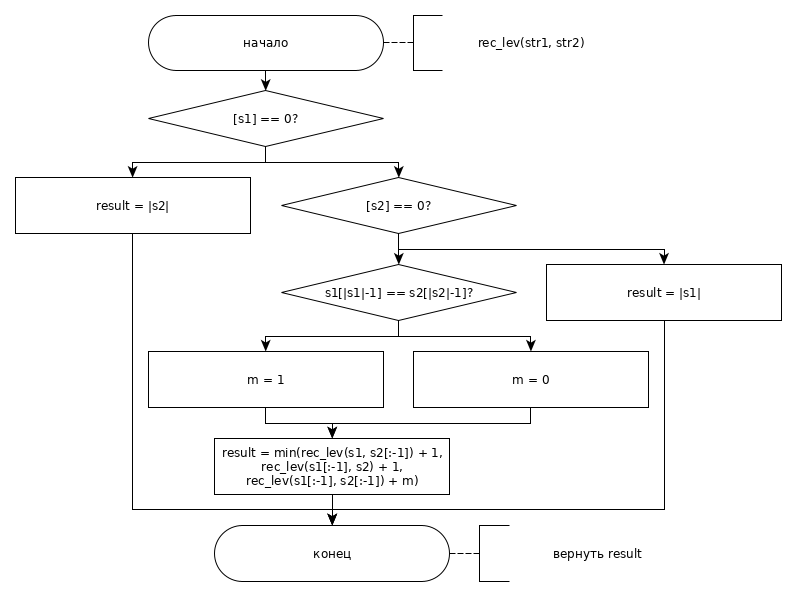
\includegraphics[scale=0.51]{lrec.png}
		 				\caption{Рекурсивный алгоритм вычисления расстояния Левенштейна}
			 			\label{ris:rec_sheme}
		 			}
		 		\end{figure}
	
	\begin{algorithm}
		\caption{Рекурсивный алгоритм вычисления расстояния Левенштейна $dist(s, t)$}
		\begin{algorithmic}
			\If{$ |s| = 0$}
				\State \Return $|t|$
			\EndIf
			\If {$ |t| = 0$}
				\State \Return $|s|$
			\EndIf
			\State $val \gets 1$
			\If {$ s[|s|] = t[|t|]$}
				\State $val \gets 0$
			\EndIf
			\State \Return $min
				\begin{cases}
					dist(s[1 \dots |s|-1], t)+1 \\
					dist(s, t[1 \dots |t|-1])+1 \\					
					dist(s[1 \dots |s|-1], t[1 \dots |t|-1])+val \\			
				\end{cases}$						
		\end{algorithmic}
	\end{algorithm}
    \newpage
    
    \afterpage{\FloatBarrier}
    \subsubsection{Матричный алгоритм вычисления расстояния Левенштейна}
        На рис.~\ref{ris:matr_lev_sh1} и рис.~\ref{ris:matr_lev_sh2} представлена схема матричного алгоритма нахождения расстояния Левенштейна
		 		\begin{figure}[h]
		 			\centering
		 			{
		 				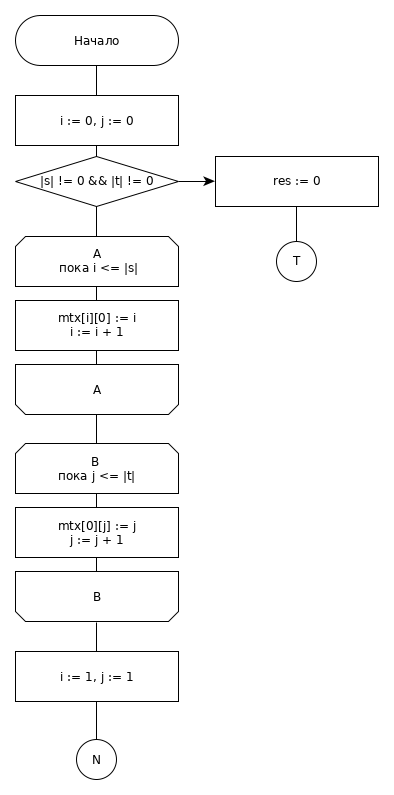
\includegraphics[scale=0.51]{lm.png}
		 				\caption{Матричный алгоритм вычисления расстояния Левенштейна}
		 				\label{ris:matr_lev_sh1}
		 			}
		 		\end{figure}
		 		\begin{figure}[h]
		 			\centering
		 			{
		 				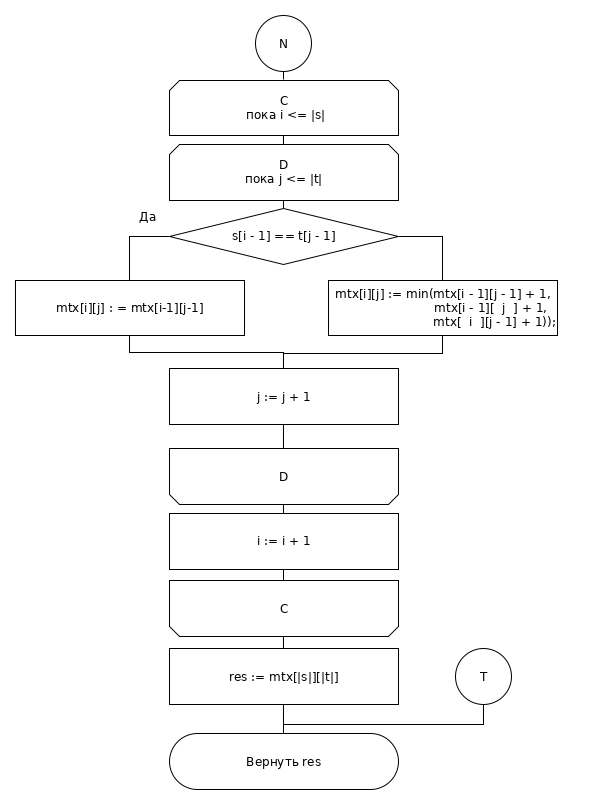
\includegraphics[scale=0.51]{lm2.png}
		 				\caption{Матричный алгоритм вычисления расстояния Левенштейна}
		 				\label{ris:matr_lev_sh2}
		 			}
		 		\end{figure}	
	\begin{algorithm}
		\caption{Матричный алгоритм вычисления расстояния Левенштейна $dist(s, t)$}
		\begin{algorithmic}
			\State $mtx [0 \dots n, 0 \dots m] \gets 0$
			
			\For{\textbf{от} $i=0$ \textbf{из} [0 \dots m]}
				\State $mtx[0, i] \gets i$
			\EndFor
			\For{\textbf{от} $i=1$ \textbf{из} [1 \dots n]}
				\State $mtx[i, 0] \gets i$
			\EndFor
			\State
			\For{\textbf{от} $i=0$ \textbf{из} [0 \dots n]}
				\For{\textbf{от} $j=0$ \textbf{из} [0 \dots m]}
					\If {$ s[i] = t[j]$}
						\State $mtx[i, j] = mtx[i-1, j-1]$
					\Else
						\State $mtx[i, j] = min(mtx[i,j-1]+1, mtx[i-1][j]+1,mtx[i-1,j-1]+1)$
					\EndIf
				\EndFor
			\EndFor
			\State \Return $mtx[m, n]$
				
		\end{algorithmic}
	\end{algorithm}
    \newpage	
    
    \afterpage{\FloatBarrier}
    \subsubsection{Матричный алгоритм вычисления расстояния Левенштейна}
            На рис.~\ref{ris:matr_dl_sh1} и рис.~\ref{ris:matr_dl_sh2} представлена схема матричного алгоритма нахождения расстояния Левенштейна
\begin{figure}[h]
		 			\centering
		 			{
		 				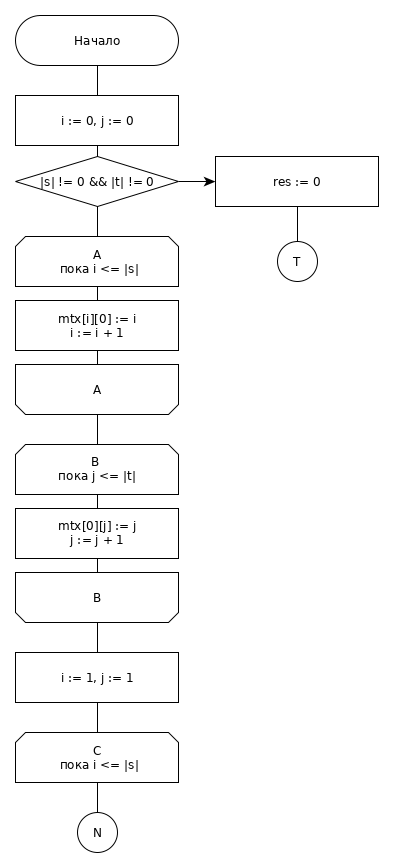
\includegraphics[scale=0.51]{dlm.png}
		 				\caption{Матричный алгоритм вычисления расстояния Дамерау-Левенштейна}
		 				\label{ris:matr_dl_sh1}
		 			}
		 		\end{figure}
		 		\begin{figure}[h]
		 			\centering
		 			{
		 				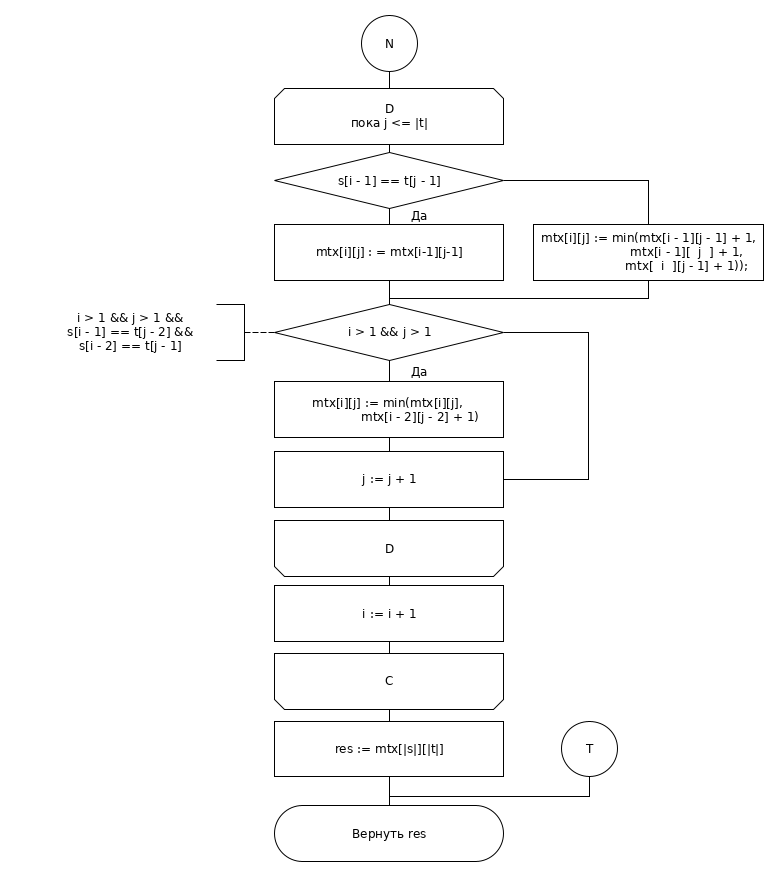
\includegraphics[scale=0.51]{dlm2.png}
		 				\caption{Матричный алгоритм вычисления расстояния Дамерау-Левенштейна}
		 				\label{ris:matr_dl_sh2}
		 			}
		 		\end{figure}
	
	\begin{algorithm}
		\caption{Матричный алгоритм вычисления расстояния Дамерау-Левенштейна $dist(s, t)$}
		\begin{algorithmic}
			\State $mtx [0 \dots n, 0 \dots m] \gets 0$
			
			\For{\textbf{от} $i=0$ \textbf{из} [0 \dots m]}
				\State $mtx[0, i] \gets i$
			\EndFor
			\For{\textbf{от} $i=1$ \textbf{из} [1 \dots n]}
				\State $mtx[i, 0] \gets i$
			\EndFor
			
			\State
			
			\For{\textbf{от} $i=0$ \textbf{из} [0 \dots n]}
				\For{\textbf{от} $j=0$ \textbf{из} [0 \dots m]}
					\If {$ s[i] = t[j]$}
						\State $mtx[i, j] = mtx[i-1, j-1]$
					\Else
						\State $mtx[i, j] = min(mtx[i,j-1]+1, 
												mtx[i-1][j]+1,
												mtx[i-1,j-1]+1)$
					\EndIf
					\If {$i > 1 и j > 1 и s[i-1]=t[j-2] и s[i-2]=t[j-1]$}
						\State $mtx[i,j] = min(mtx[i,j], mtx[i-2,j-2]+1)$
					\EndIf 
				\EndFor
			\EndFor
			\State \Return $mtx[m, n]$
				
		\end{algorithmic}
	\end{algorithm}
    \newpage
    \afterpage{\FloatBarrier}
    \begin{center}
    	\subsection{Выводы по конструкторскому разделу}    
    \end{center}
   
    	\qquad Были разработаны схемы трех алгоритмов вычисления расстояния Левенштейна и его модификации, алгоритма Дамерау-Левенштейна. Каждый из них был описан с помощью псевдокода.
    	
    \newpage
    
    \begin{center}
     	\section{Технологическая часть}
    	\subsection{Требования к программному обеспечению}
    \end{center}
    
    	\quad Программа должна работать в одном из двух режимов: пользовательском и эксперементальном.\\
    	В пользовательском режиме должны быть реализованы: 
    	
    	\begin{itemize}
    		\item ввод исходных данных с клавиатуры 
    		\item вывод результата работы алгоритмов 
    		\item отсутствие аварийных ситуаций
    	\end{itemize}
		Эксперементальный режим должен также предоставлять сведенья о затраченном на выполнение алгоритмов процессорном времени.
    \begin{center}
        \subsection{Средства реализации}    
    \end{center}
    
		В качестве языка программирования был выбран C++, так как он предоставляет широкие возможности для эффективной реализации алгоритмов.
	\begin{center}
	\end{center}
	\begin{center}
		\subsection{Структура программы}	
		\end{center}
	
    	\noindent levenshtain\_dist.cpp - содержит реализацию алгоритмов поиска расстояния Левенштейна и Дамерау-Левенштейна\\
    	test.cpp - содержит тесты для реализованных алгоритмов\\
	    main.cpp - содержит интерфейс для взаимодействия с программой\\
		\newpage
    \begin{center}
        \subsection{Листинг кода}    
    \end{center}
\lstset{
	        		language=C++,
	        		basicstyle=\ttfamily,
	        		keywordstyle=\color{blue}\ttfamily,
	        		stringstyle=\color{red}\ttfamily,
	        		commentstyle=\color{green}\ttfamily,
	        		morecomment=[l][\color{magenta}]{\#},
	        		columns=fullflexible,
	        	    tabsize=1, 
	        		breakatwhitespace=true
	        	}
        	
        		\begin{lstlisting}[frame=single,caption=Рекурсивный алгоритм вычисления расстояния Левенштейна, breaklines]
int recursive_lev(std::string str1, std::string str2) {
    auto len1 = str1.length();
    auto len2 = str2.length();

    if (len1 == 0) {
        return static_cast<int>(len2);
    }
    if (len2 == 0) {
        return static_cast<int>(len1);
    }

    auto last_symb = str1[len1 - 1] == str2[len2 - 1]? 0: 1;

    auto s1 = std::string(str1, 0, len1 - 1);
    auto s2 = std::string(str2, 0, len2 - 1);

    return std::min( { recursive_lev(str1, s2) + 1,
                       recursive_lev(s1, str2) + 1,
                       recursive_lev(s1, s2) + last_symb });
}
        		\end{lstlisting}        		
    
            	\begin{lstlisting}[frame=single,caption=Матричный алгоритм вычисления расстояния Левенштейна, breaklines]
int lev(std::string str1, std::string str2) {
    std::vector<int> a1(str2.length() + 1);
    std::vector<int> a2(str2.length() + 1);
    // initialisation of 1st row
    for (int i = 0; i < a1.size(); i++) a1[i] = i;

    for (int i = 1; i < str1.length() + 1; i++) {
        a2.at(0) = a1.at(0) + 1;
        for (int j = 1; j < str2.length() + 1; j++) {
            auto vertical = a1[j] + 1;
            auto horisontal = a2[j - 1] + 1;
            auto diagonal = a1[j - 1] + (str1[i - 1] == str2[j - 1]? 0: 1);
            a2[j] = std::min({ vertical, horisontal, diagonal });
        }
        std::copy(a2.begin(), a2.end(), a1.begin());
    }

    return a2[a2.size() - 1];
}
   				 \end{lstlisting}
    \newpage
            	\begin{lstlisting}[frame=single,caption=Матричный алгоритм вычисления расстояния Дамерау-Левенштейна, breaklines]
int dam_lev_dist(std::string str1, std::string str2) {
    std::vector<int> a0(str2.length() + 1);
    std::vector<int> a1(str2.length() + 1);
    std::vector<int> a2(str2.length() + 1);
    // initialisation of 1st row
    for (int i = 0; i < a1.size(); i++) a1[i] = i;

    for (int i = 1; i < str1.length() + 1; i++) {
        a2[0] = a1[0] + 1;
        for (int j = 1; j < str2.length() + 1; j++) {
            auto eq = str1[i - 1] == str2[j - 1]? 0: 1;

            auto vertical = a1[j] + 1;
            auto horisontal = a2[j - 1] + 1;
            auto diagonal = a1[j - 1] + eq;
            a2[j] = std::min({ vertical, horisontal, diagonal });

            // swap
            if (i && j && str1[i - 1] == str2[j - 2] 
            	&& str1[i - 2] == str2[j - 1]) {
                a2[j] = std::min(a2[j], a0[j - 2] + eq);
            }
        }
        a0 = a1;
        a1 = a2;
    }

    return a2[a2.size() - 1];
}
				\end{lstlisting}
    \newpage
    \begin{center}
		\subsection{Тестирование фунций}
	\end{center}
		\quadВ таблице ~\ref{tabular:test_rec}, таблице~\ref{tabular:test_mtrx_l}, таблице~\ref{tabular:test_mtrx_dl} приведены результаты тестирования для рекурсивного, матричного алгоритмов вычисления расстояния Левенштейна и алгоритма нахождения расстояния Дамерау-Левенштейна соответственно.
        			\begin{table}[H]        		
       				\caption{\label{tabular:test_rec} Рекурсивный алгоритм вычисления расстояния Левенштейна}
       				\begin{center}       			
        			\begin{tabular}{|c|c|c|c|}        				
        				\hline
						Строка 1 & Строка 2 & Результат & Ожидаемый результат \\ 
						\hline
        				kot    & skat  & 2  & 2\\
        				abc  & abc &0  & 0\\
        				kot  & null  & 3  & 3\\
        				null  & kot  & 3  & 3\\
        				null  & null  & 0  & 0\\
        				abc  & acb  & 2 & 2\\
        				\hline
        			\end{tabular}
       				\end{center}
        			\end{table}        			
        			%Таблица 1.
        			\vspace{1.5cm}
        		
        			\begin{table}[H]        		
       				\caption{\label{tabular:test_mtrx_l} Матричный алгоритм вычисления расстояния Левенштейна}
       				\begin{center}
        			\begin{tabular}{|c|c|c|c|}        		
						\hline
        				Строка 1 & Строка 2 &Результат &Ожидаемый результат \\ 							\hline
        				kot    &skat  &2  &2\\
        				abc  &abc &0  &0\\
        				kot  &null  &3  &3\\
        				null  &kot  &3  &3\\
        				null  &null  &0  &0\\
        				abc  &acb  &2 &2\\ 
        				\hline        				
        			\end{tabular}
        			\end{center}
        			\end{table}
        			\vspace{1.5cm}
        		
					\begin{table}[H]        		
       				\caption{\label{tabular:test_mtrx_dl} Матричный алгоритм вычисления расстояния Дамерау-Левенштейна}
       				\begin{center}       			
        			\begin{tabular}{|c|c|c|c|}        			
        				\hline
        				Строка 1 & Строка 2 &Результат &Ожидаемый результат \\ 							\hline
        				kot    &skat  &2  &2\\
        				abc  &abc &0  &0\\
        				kot  &null  &3  &3\\
        				null  &kot  &3  &3\\
        				null  &null  &0  &0\\
        				abc  &acb  &1 &1\\ 
        				\hline
        			\end{tabular}
       				\end{center}
	        		\end{table}
	\newpage

    \begin{center}
        \section{Экспериментальная часть}
        \subsection{Примеры работы}
    \end{center}
    
   	\smallskip
	\noindent{\it \textbf{Входные данные: }}\\
	\smallskip
	Enter 1st string: \textbf{kot}\\
	Enter 2nd string: \textbf{skat}\\
	Run time tests? y \slash n? \textbf{n}
	
	\noindent{\it \textbf{Выходные данные: }}\\
	\smallskip
	\noindent Levenshtein distance (Matrix)\\
	Matrix:\\
    -   $\lambda$   q   w   e\\
    $\lambda$   0   1   2   3\\
    a   1   1   2   3\\
    d   2   2   2   3\\
    e   3   3   3   3

    \noindent Result: 3


	\noindent Levenshtein distance (Recursive)\\
	Result: 3


	\noindent Damerau-Levenshtein distance (Matrix)\\
	Matrix:\\
    -   $\lambda$   q   w   e\\
    $\lambda$   0   1   2   3\\
    a   1   1   2   3\\
    d   2   2   2   3\\
    e   3   3   3   3

	\noindent Result: 3\\
	
	\smallskip
	\noindent{\it \textbf{Входные данные: }}\\
	\smallskip
	Enter 1st string: \textbf{kot}\\
	Enter 2nd string: \textbf{skat}\\
	Run time tests? y \slash n? \textbf{y}
	
	\noindent{\it \textbf{Выходные данные: }}\\
	\smallskip
	\noindent Levenshtein distance (Matrix)\\
	Time: 0.00001110s\\
	Matrix:\\
    -   $\lambda$   q   w   e\\
    $\lambda$   0   1   2   3\\
    a   1   1   2   3\\
    d   2   2   2   3\\
    e   3   3   3   3

    \noindent Result: 3


	\noindent Levenshtein distance (Recursive)\\
	Time: 0.00004630s\\
	Result: 3


	\noindent Damerau-Levenshtein distance (Matrix)\\
	Time: 0.00001550s\\
	Matrix:\\
    -   $\lambda$   q   w   e\\
    $\lambda$   0   1   2   3\\
    a   1   1   2   3\\
    d   2   2   2   3\\
    e   3   3   3   3

	\noindent Result: 3
	\newpage
	\begin{center}
	    \subsection{Тестирование времени работы функций}	
	\end{center}
	    \quadДля измерения времени использовалась функция clock(). Чтобы исключить случайные отклонения в измеренном времени, измерялось время работы 50 запусков функции и делилось на 50.
	    
	    В таблице~\ref{tabular:test_time} представлены результаты замеров времени работы реализованных алгоритмов. На рис.~\ref{ris:cmp_mtrx} и рис.~\ref{ris:cmp_r_and_m} изображены графики, позволяющие сравнить эффективность реализаций.
	\begin{table}[H]
	\caption{\label{tabular:test_time} Время работы реализаций алгоритмов}
	\begin{center}	    
	\begin{tabular}{|c|c|c|c|c|}
        				
        				\hline
        				|Строка 1| & |Строка 2| &МДЛ      &МЛ        &РЛ\\ 
        				\hline
        				200      &200       &0.002242 &0.002173  &-\\
        				100      &100       &0.000867 &0.000848  &-\\
        				50       &50        &0.000545 &0.000607  &-\\
        				10       &10        &0.000045 &0.000041  &0.430871\\ 
        				8        &8         &0.000031 &0.000028  &0.017353\\
        				5        &5         &0.000018 &0.000015  &0.000689\\ 
        				50       &2         &0.000042 &0.000048  &0.001515\\
        				50       &4         &0.000123 &0.000114  &0.283745\\
        				\hline
	\end{tabular}
	\end{center}
	\end{table}	
	
	\begin{center}
	\begin{figure}[h]	
        				{
        					\centering
        					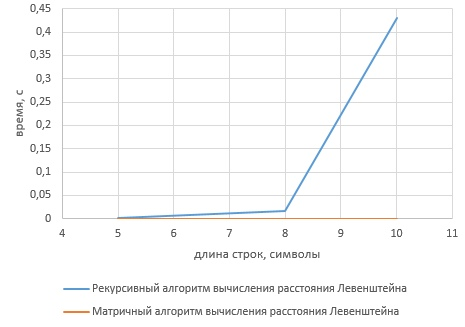
\includegraphics[scale=0.7]{t1.jpg}
        					\caption{Сравнение матричных реализаций алгоритмов}
        					\label{ris:cmp_mtrx}
        				}
        			\end{figure}
        		
        			\begin{figure}[h]	
        				{
        					\centering
        					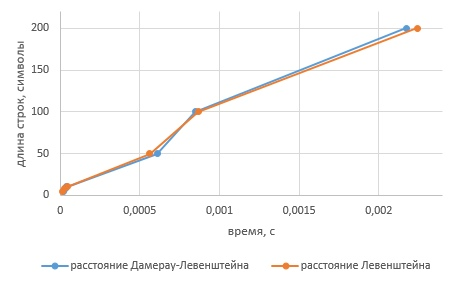
\includegraphics[scale=0.7]{t2.jpg}
        					\caption{\label{ris:cmp_r_and_m}Сравнение рекурсивного и матричного алгоритма}        					
        				}
        			\end{figure}
	\end{center}
	\newpage
	Время работы матричных реализаций практически не отличается друг от друга, а рекурсивная реализация алгоритма нахождения реализации Левенштейна уже на строках длины 9 работает медленнее в 500 раз.

    \newpage

    \begin{center}
        \section*{Заключение}
        \addcontentsline{toc}{section}{Заключение}
    \end{center}
            \label{sec:ending}
        	\qquad В рамках лабораторной работы были реализованы и изучены рекурсивный алгоритм нахождения расстояния Левенштейна, матричная версия алгоритма и алгоритм нахождения расстония Дамерау-Левенштейна. Были произведены замеры времени работы реализованных алгоритмов и сравнена их эффективность по времени и памяти. Матричные алгоритмы оказались близки по эффективности, рекурсивный алгоритм же работает значительно медленнее матричных реализаций, уже при длинне строк больше 10 установить время работы не удалось.

    \newpage

    \begin{center}        
        \begin{thebibliography}{}
        	\bibitem{litlink5}  В. И. Левенштейн. Двоичные коды с исправлением выпадений, вставок и замещений символов. Доклады Академий Наук СССР, 1965. 163.4:845-848.
        	\bibitem{litlink3}  Damareau , F., J., "A technique for computer detection and correction of spelling errors"
			
        	
        	\bibitem{litlink2}  Ovicic, V., "Constrained edit distance algorithm and its application in Library Information Systems"           
			\bibitem{litlink4}  The Institute of Electronics, "Tree Edit Distance Problems: Algorithms and Applications to Bioinformatics"
        	\bibitem{litlink6}  Гасфилд. Строки, деревья и последовательности в алгоритмах. Информатика и вычислительная биология. Невский Диалект БВХ-Петербург, 2003.
        	        	
        	\bibitem{litlink1}	US National Library of Medicine National Institutes of Health, "Secure approximation of edit distance on genomic data"
        	 	
        	
        \end{thebibliography}
    \end{center}

\end{document}
